\chapter{Polarity classification}
\label{polarity}

Given that we can now determine whether a status contains an opinion, the next stage within our sentiment analysis engine lies in determining the status' polarity. Polarity classification specifically looks at determining whether a status is \emph{positive}, \emph{negative} or in some cases \emph{neutral}. Approaches to classifying polarity have typically been supervised. This is largely due to the difficulty of identifying the numerous nuanced linguistic details which could imply polarity. Although some \cite{Turney:2002vv} have attempted un-supervised approaches, recent work such as that covered by Liu \cite{Liu:2010tm} shows that there is a much greater deal of success when supervised techniques are applied. Accordingly, we elected to take a supervised approach for polarity classification, with the hope that we might also be able to draw upon some of the linguistic insight offered by unsupervised approaches.

In this chapter we shall first examine how we labelled and annotated our training set, before going on to explore our choice of potential features and their implementations. Next we shall discuss the results of our testing and explain our choice of features, before finally evaluating the success of our classifier with particular respect to prior research.

\section{Training set}

Our approach to polarity classification will take a two-label approach similar to that proposed by Pang et al. \cite{Pang:2002tu}. Thus each \emph{TrainedStatus} object will be annotated with a \texttt{polarity} attribute of either "positive" or "negative". Furthermore, we will expand upon our original subjectivity annotations in order to collect phrases which are not only subjective, but positive or negative. In order to do this, we will define two additional attributes \texttt{positive\-\_clues} and \texttt{negative\-\_clues}. Both of these will be used to store any positive or negative phrases that might occur within the status being annotated.

Thus, for each \emph{TrainedStatus} object, we now have three additional attributes, \texttt{polarity}, \texttt{positive\-\_clues} and \texttt{negative\-\_clues}.

\section{Features}

In order to build an accurate polarity classifier, selecting discriminative features is fundamental. Within our approach we shall draw upon those which have been shown to be successful within literature. Furthermore we shall also look at experimenting with aspects of un-supervised techniques as new and previously untested potential features. The remainder of this section shall focus on our feature implementation, and we shall save a discussion of their effectiveness till our results section.

\subsection{Unigrams}

As noted by Pang and Lee \cite{Pang:2002tu}, unigrams can often serve as strong discriminative features when classifying polarity. In effect unigrams provide a presence feature for all possible words, however their implementation means that this set of words is limited to those seen when training the classifier, rather than the actual set of all possible words.

As the implementation for unigrams is so distinct from other features, its feature code was built directly into the \emph{Classifier} class, rather than our \emph{PolarityClassifier} class. In order to build our unigrams, we require a two stage process. Before training occurs our unigram set is initialised by iterating through each status, adding its words to our unigram set.  When added, words' are down-cased in order to avoid adding the same word multiple times. Once finished we have an array consisting of every single word used in all of our training examples.

When building a status' feature set either for training or classification, we make use of the previously built array of unigram words. For every word in the unigram array, a feature is added to the status' feature set denoting whether the said word occurs within the status. In order to do this we built a \texttt{parse\_unigram(status)} method, which when given a status, will return the corresponding unigram feature set, as shown in listing \ref{polarity:unigrams}.

\begin{lstlisting}[language=Ruby, caption={\emph{Classifier} class' \texttt{parse\_unigram} method.}, label=polarity:unigrams]
def parse_unigrams status
	# downcases and collects every word within the status
  words = status.parts_of_speech.map{|p| p["word"].downcase}
	# iterates over the array of unigram words, noting whether the unigram exists within our status' set of words 
  self.unigrams.map{|u| words.include?(u) ? 1 : 0}
end
\end{lstlisting}

Alongside the \texttt{parse\-\_unigram\-(status)} method, we introduced two other methods. The \texttt{parse\-\_hashtag\-\_unigram\-(status)} produces a unigram feature set in which only hashtags are used as unigrams feature. An additional, more detailed method, \texttt{parse\-\_pos\-\_unigram\-(status)} creates a feature for every word and part of speech tag combination.

In order to simplify the process of including unigrams in our feature set, our classifiers can be initialised with any combination of the three unigram-based features below, just as we would with a normal features. If any of them are included, their corresponding method is called, and the resultant feature set is added to the status' overall feature set. These three methods are:

\begin{description}
	\item [\texttt{unigrams}] is our primary unigram feature. It calls the \texttt{parse\-\_unigram\-(status)} for any given status, and appends the resultant feature set to the status' overall feature set.
	\item [\texttt{hashtag\_unigrams}] builds a unigram feature set which inly acknowledges hashtags as words. It calls the \texttt{parse\-\_hashtag\-\_unigram\-(status)} for any given status, and appends the resultant feature set to the status' overall feature set.
	\item [\texttt{unigrams\_pos}] builds a more specific unigram feature set than \texttt{unigrams} in which each unigram is a combination of both the word and part of speech it represents. Thus, rather than only checking each word in a status, it will instead check each word and part of speech combination in a status. It calls the \texttt{parse\-\_pos\-\_unigram\-(status)} for any given status, and appends the resultant feature set to the status' overall feature set.
\end{description}

In order to help clarify how the \texttt{parse\-\_unigram\-(status)} method works, an example has been given in listing \ref{polarity:unigram_output}.

\begin{lstlisting}[language=Ruby, caption={Unigram parsing for \emph{Example 1} using a small unigram set}, label=polarity:unigram_output]
# let status = Example 1
# let self.unigrams = [think, hate, love, good, bad, strong, weak]
parse_unigrams status
	=> [1,0,0,1,0,1,0]
\end{lstlisting}

\subsection{Polarity clues}
\label{polarity:clues}

Polarity clues are used to identify terms which express polarised opinion. This is a core feature of most polarity classifiers, although the approaches to determining whether a word is polarised vary. We will again draw upon the work of Wiebe and Riloff \cite{Wiebe:2003wa} using chapter \ref{subjectivity}'s \emph{ClueFinder} class. In addition to using the polarised clues presented by Wiebe and Riloff, we also use our own annotated collection of clues and seed words by additionally loading them into the lexicon.

Furthermore when finding clues within a status we also look to further populate our lexicon. All adjective-conjunct-adjective trigrams are extracted, and if one of the adjectives is contained within our clue lexicon, the other is also added. If the conjunct is "\emph{and}", then the new clue is tagged with the same polarity as the existing clue, and if the conjunct used is "\emph{but}" the new clue's polarity is set to the opposite of the existing clue's. Using this un-supervised technique, we are able to further populate our lexicon with no additional effort. This is run on all input statuses, thus it is assumed that the lexicon will improve with time. 

Using our \emph{ClueFinder}'s original \texttt{clue\_data} method we define an additional four methods for our \emph{Status} object, \texttt{weak\-\_positive\-\_clues}, \texttt{strong\-\_positive\-\_clues}, \texttt{weak\-\_negative\-\_clues} and \texttt{strong\-\_negative\-\_clues}. In order to handle negation within these methods, whenever a negation word such as "not" is encountered, all words up to the next grammatical punctuation are inverted. For further implementation detail please refer to listing \ref{polarity:polarised_clues}. Each of these are then used to help define twelve new clue-based feature methods. We will define only the first four, as the last eight are simply derivatives which introduce the concepts of \emph{weak} and \emph{strong} clues.

\begin{description}
	\item [\texttt{has\_positive\_clues?}] returns a boolean value denoting the presence of one or more positive clues.
	\item [\texttt{no\_positive\_clues}] returns one of three values based upon the number of positive clues. For zero clues, \texttt{0} is returned, for one or two clues, \texttt{1} is returned and for three or more clues \texttt{2} is returned.
	\item [\texttt{has\_negative\_clues}?] as with \texttt{has\-\_positive\-\_clues?}, but only noting negative clues.
	\item [\texttt{no\_negative\_clues}] as with \texttt{no\-\_positive\-\_clues}, but only noting negative clues.
\end{description}

\subsection{Subjective patterns}

In Turney's \cite{Turney:2002vv} un-supervised approach, he proposes five grammatical structures for identifying subjective phrases. He suggest that the polarity of these phrases are in turn indicative of their sentence's overall polarity. Although we felt that as an un-supervised approach alone it was not suitable for the project, we decided to explore the possibility of using it as a feature within our supervised classification.

Each of the rules from table \ref{background:patterns} are assembled as items within a \texttt{rules} array. Each rule is encoded as an array of three arrays. The first two inner arrays contain all possible part of speech which the first two words of the phrase \emph{must} be. The last array contains all the parts of speech which the third word \emph{must not} be, as implemented in lines 2 to 8 of listing \ref{polarity:patterns}. We use \texttt{nil} instead of a third array when the third word can take on any part of speech. With a rule structure now in place, we can split our status into its individual trigrams. Each trigram is then iterated over, each time checking to see if it matches any of the rules expressed in our \texttt{rules} array. Any trigram which matches one of the five rules is added to a \texttt{patterns} array, which is returned upon method completion.

Once our patterns have been extracted we can then look for clues pertaining to their polarity. This is done by using the \emph{ClueFinder} class to determine the if and what the polarity of the first two pattern-extracted words are. Using this we define two pattern-based features\footnote{As there is typically no more than one pattern in a status, we have opted to use only presence as a feature and not the number of occurences.}:

\begin{description}
	\item [\texttt{has\_negative\_patterns?}] returns a boolean value denoting the presence of one or more pattern with a negative polarity. 
	
	\item [\texttt{has\_positive\_patterns?}] returns a boolean value denoting the presence of one or more pattern with a positive polarity. 
\end{description}

\section{Results}

Within this section we shall take a similar approach to testing as that seen in chapter \ref{subjectivity}'s results section. Again, all tests are performed using three-fold cross validation over a set of 300 labelled tweets, and repeated 30 times to ensure an accurate measure.

\subsection{Individual feature performance}

As with subjectivity, in order to build the most appropriate feature set we first decided to evaluate the performance of each individual feature on its own. In order to truly understand the performance of each feature, we decided to focus on their \emph{accuracy}, \emph{precision} and \emph{recall}. For each measure we wanted to look at not only the average, but the spread of results across the 100 repetitions. We have presented our results for each measure below, and we shall now examine the results for each measure in turn.

It is important to note that in order to present our data in a tidier fashion, we will use the following numbering system when discussing and presenting features:

\begin{longtable}{|p{0.25in}|p{1.55in}|p{0.25in}|p{1.55in}|}
	
		\hline
		No. & Feature & No. & Feature \\
		\hline
		1 & has\-\_positive\-\_clues? & 9 & no\-\_weak\-\_positive\-\_clues \\
		\hline
    2 & has\-\_negative\-\_clues? & 10 & no\-\_weak\-\_negative\-\_clues \\
		\hline
    3 & has\-\_weak\-\_positive\-\_clues? & 11 & no\-\_strong\-\_positive\-\_clues \\
		\hline
    4 & has\-\_weak\-\_negative\-\_clues? & 12	& no\-\_strong\-\_negative\-\_clues \\
		\hline
    5 & has\-\_strong\-\_positive\-\_clues? & 13	& has\-\_positive\-\_patterns? \\
		\hline
		6 & has\-\_strong\-\_negative\-\_clues? & 14	& has\-\_negative\-\_patterns? \\
		\hline
		7	& no\-\_positive\-\_clues & 15	& unigrams \\
		\hline
		8	& no\-\_negative\-\_clues & 16 & hashtag\-\_unigrams \\
		\hline
		& & 17 & unigrams\-\_pos \\
		\hline
\end{longtable}
`
In figures \ref{fig:polarity_a}, \ref{fig:polarity_p} and \ref{fig:polarity_r} we present the test results for each of our single-feature classifiers.'

\begin{figure}
	\caption{Accuracy average and spread for each individual feature}
	\label{fig:polarity_a}
	\centering
		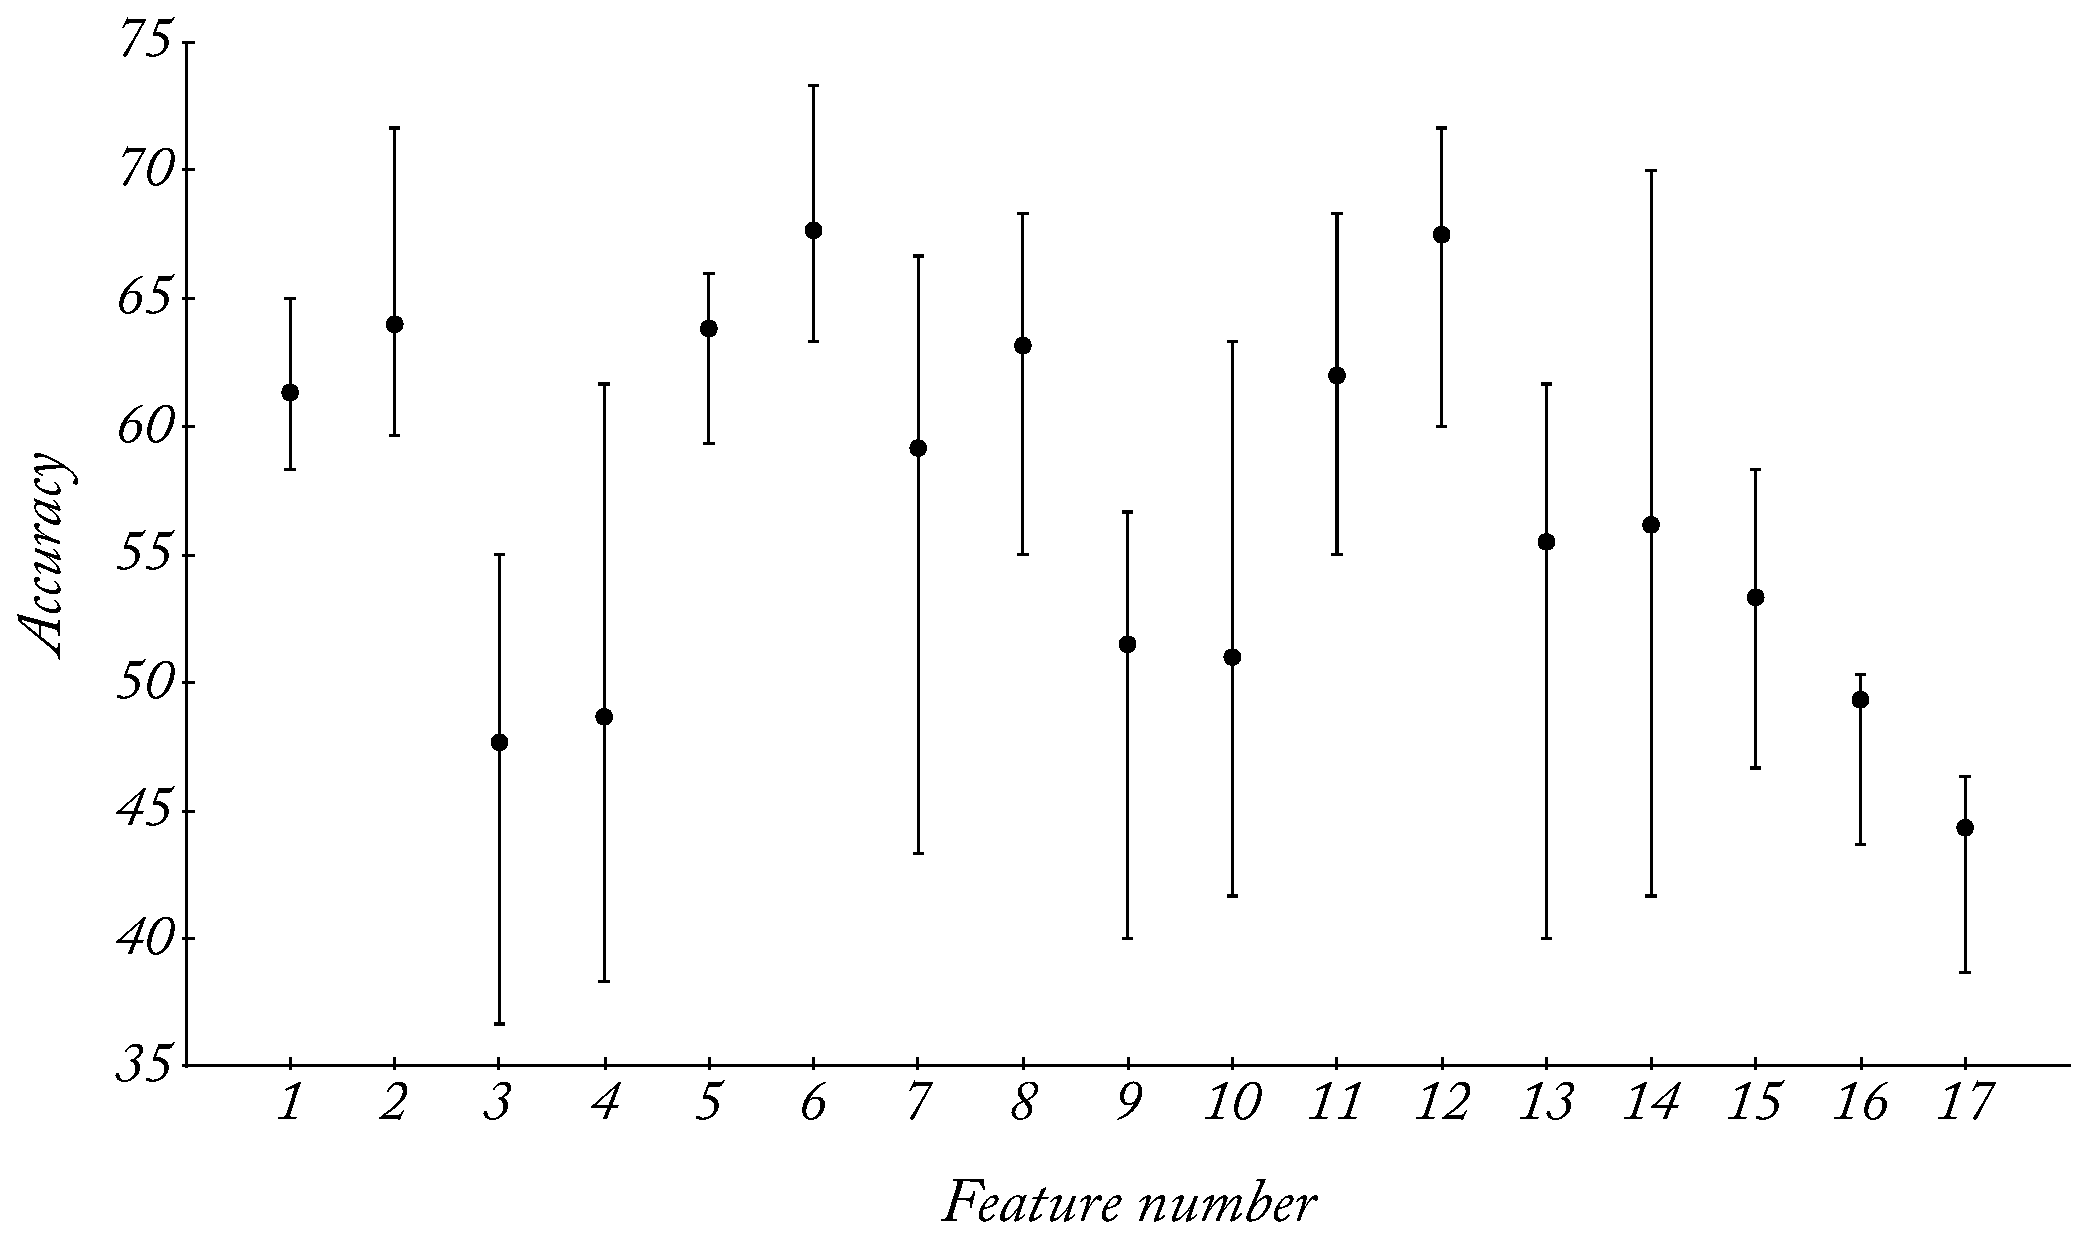
\includegraphics[width=1.0\textwidth]{graphs/polarity_a.pdf}
\end{figure}

The results across our features is not only varied in terms of accuracy but also in terms of sensitivity to changes in training data. General clue presence along with strong-clue presence/occurrence performed well, achieving strong average classification accuracies of around 65\%. Furthermore general-clue and strong-clue presence features both resulted in low spreads, suggesting a resilience to changes in training data. Interestingly, unigrams offer little more than a slight improvement above the baseline expectancy of 50\%. Some features such as the two other unigram-based features along with the four variations of weak clues all perform poorly scoring below 50\%.

\begin{figure}
	\caption{Precision average and spread for each individual feature}
	\label{fig:polarity_p}
	\centering
		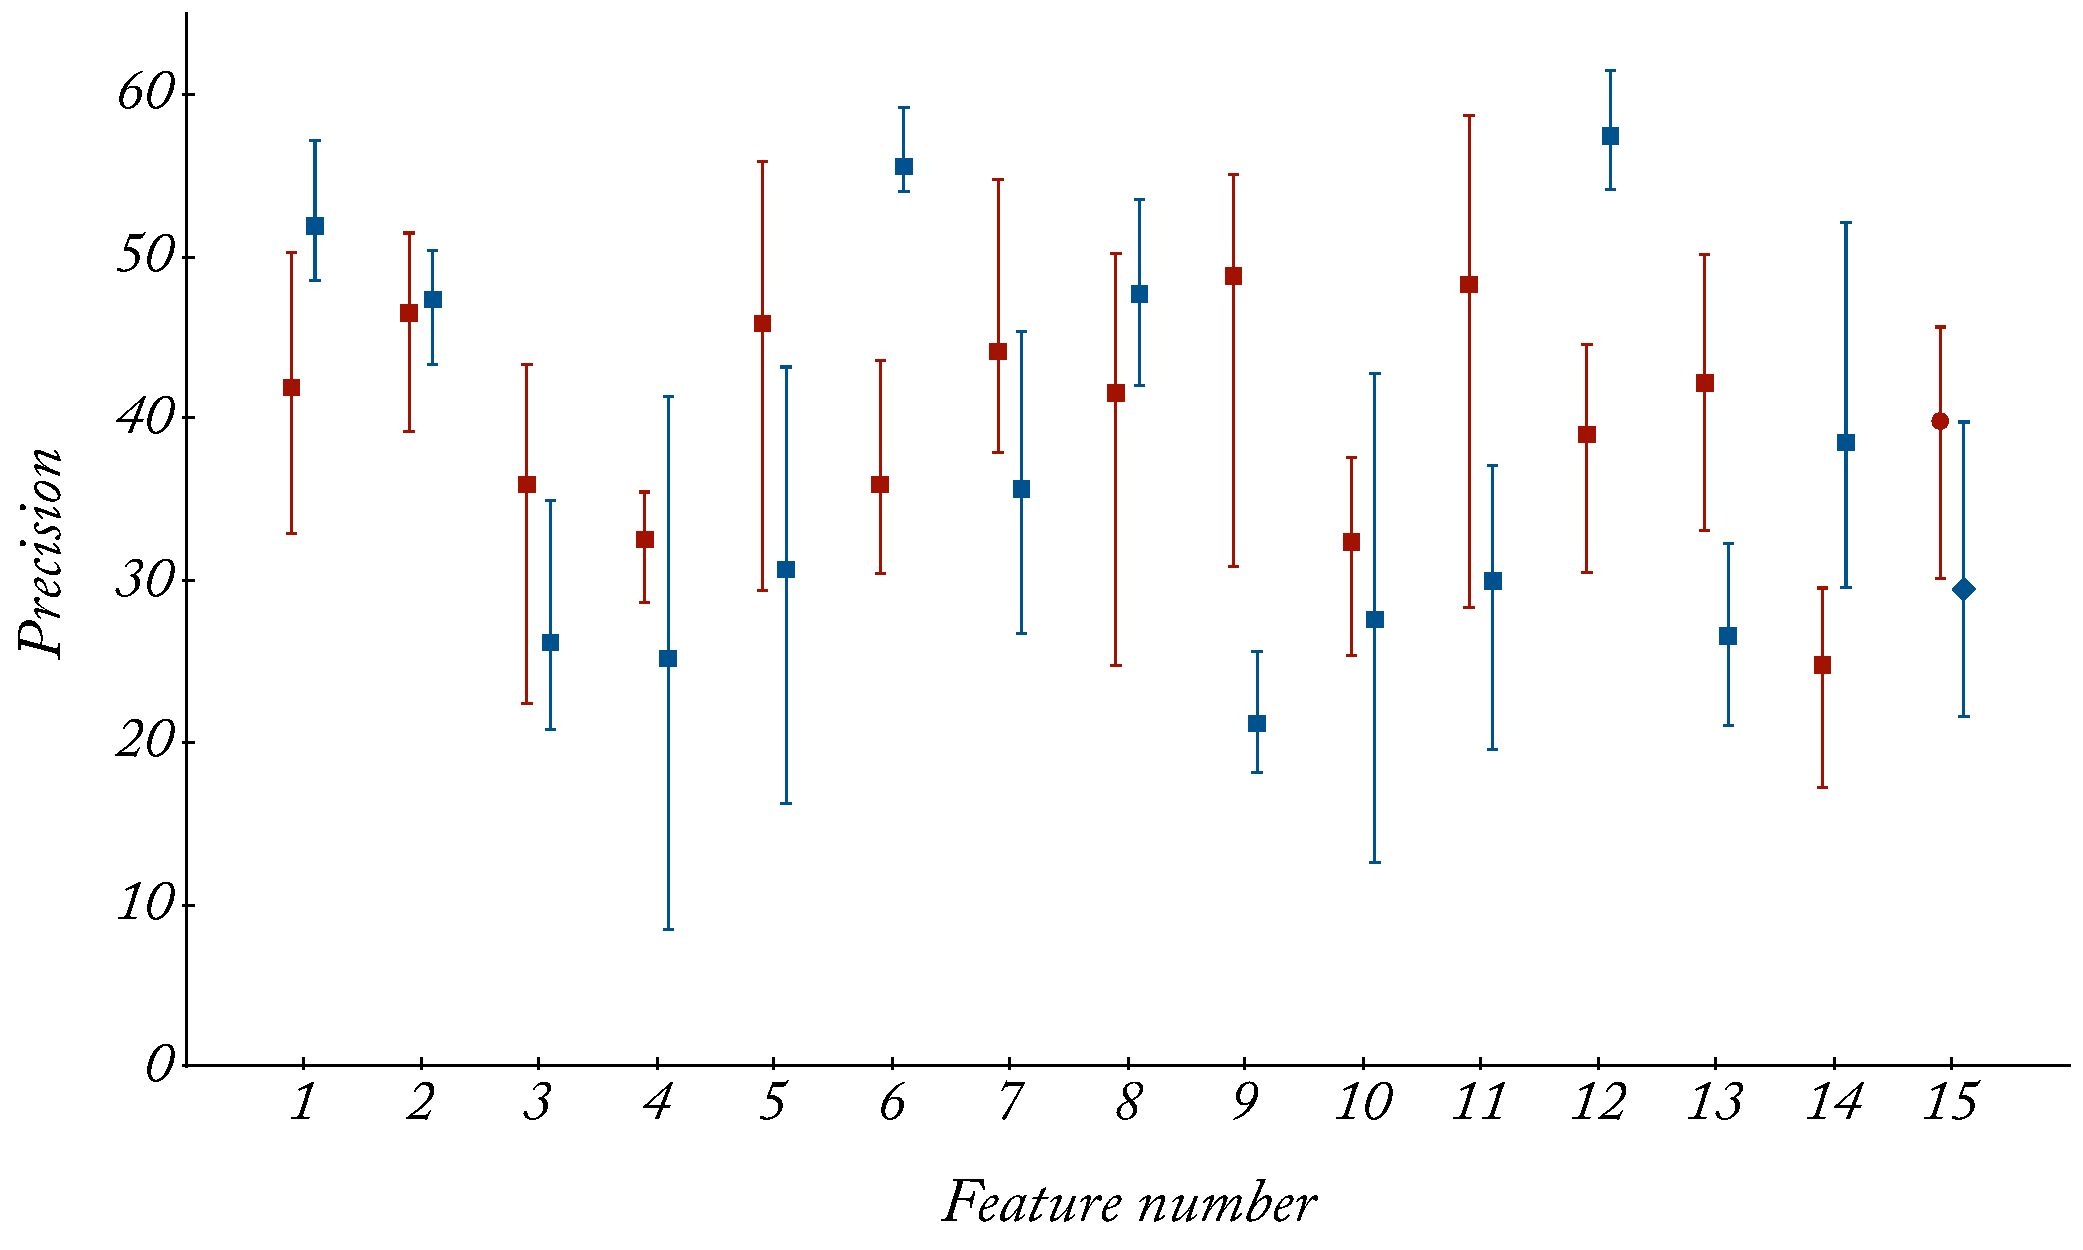
\includegraphics[width=1.0\textwidth]{graphs/polarity_p.pdf}
\end{figure}

Our precision results again highlight the benefits of using strong clues as a feature. Furthermore clue presence performs fairly well. Of particular interest however is the high precision rate seen with our pattern matched clues, suggesting that although their accuracy may be low as a whole, they're ability to classify precisely makes them a useful feature.

\begin{figure}
	\caption{Recall average and spread for each individual feature}
	\label{fig:polarity_r}
	\centering
		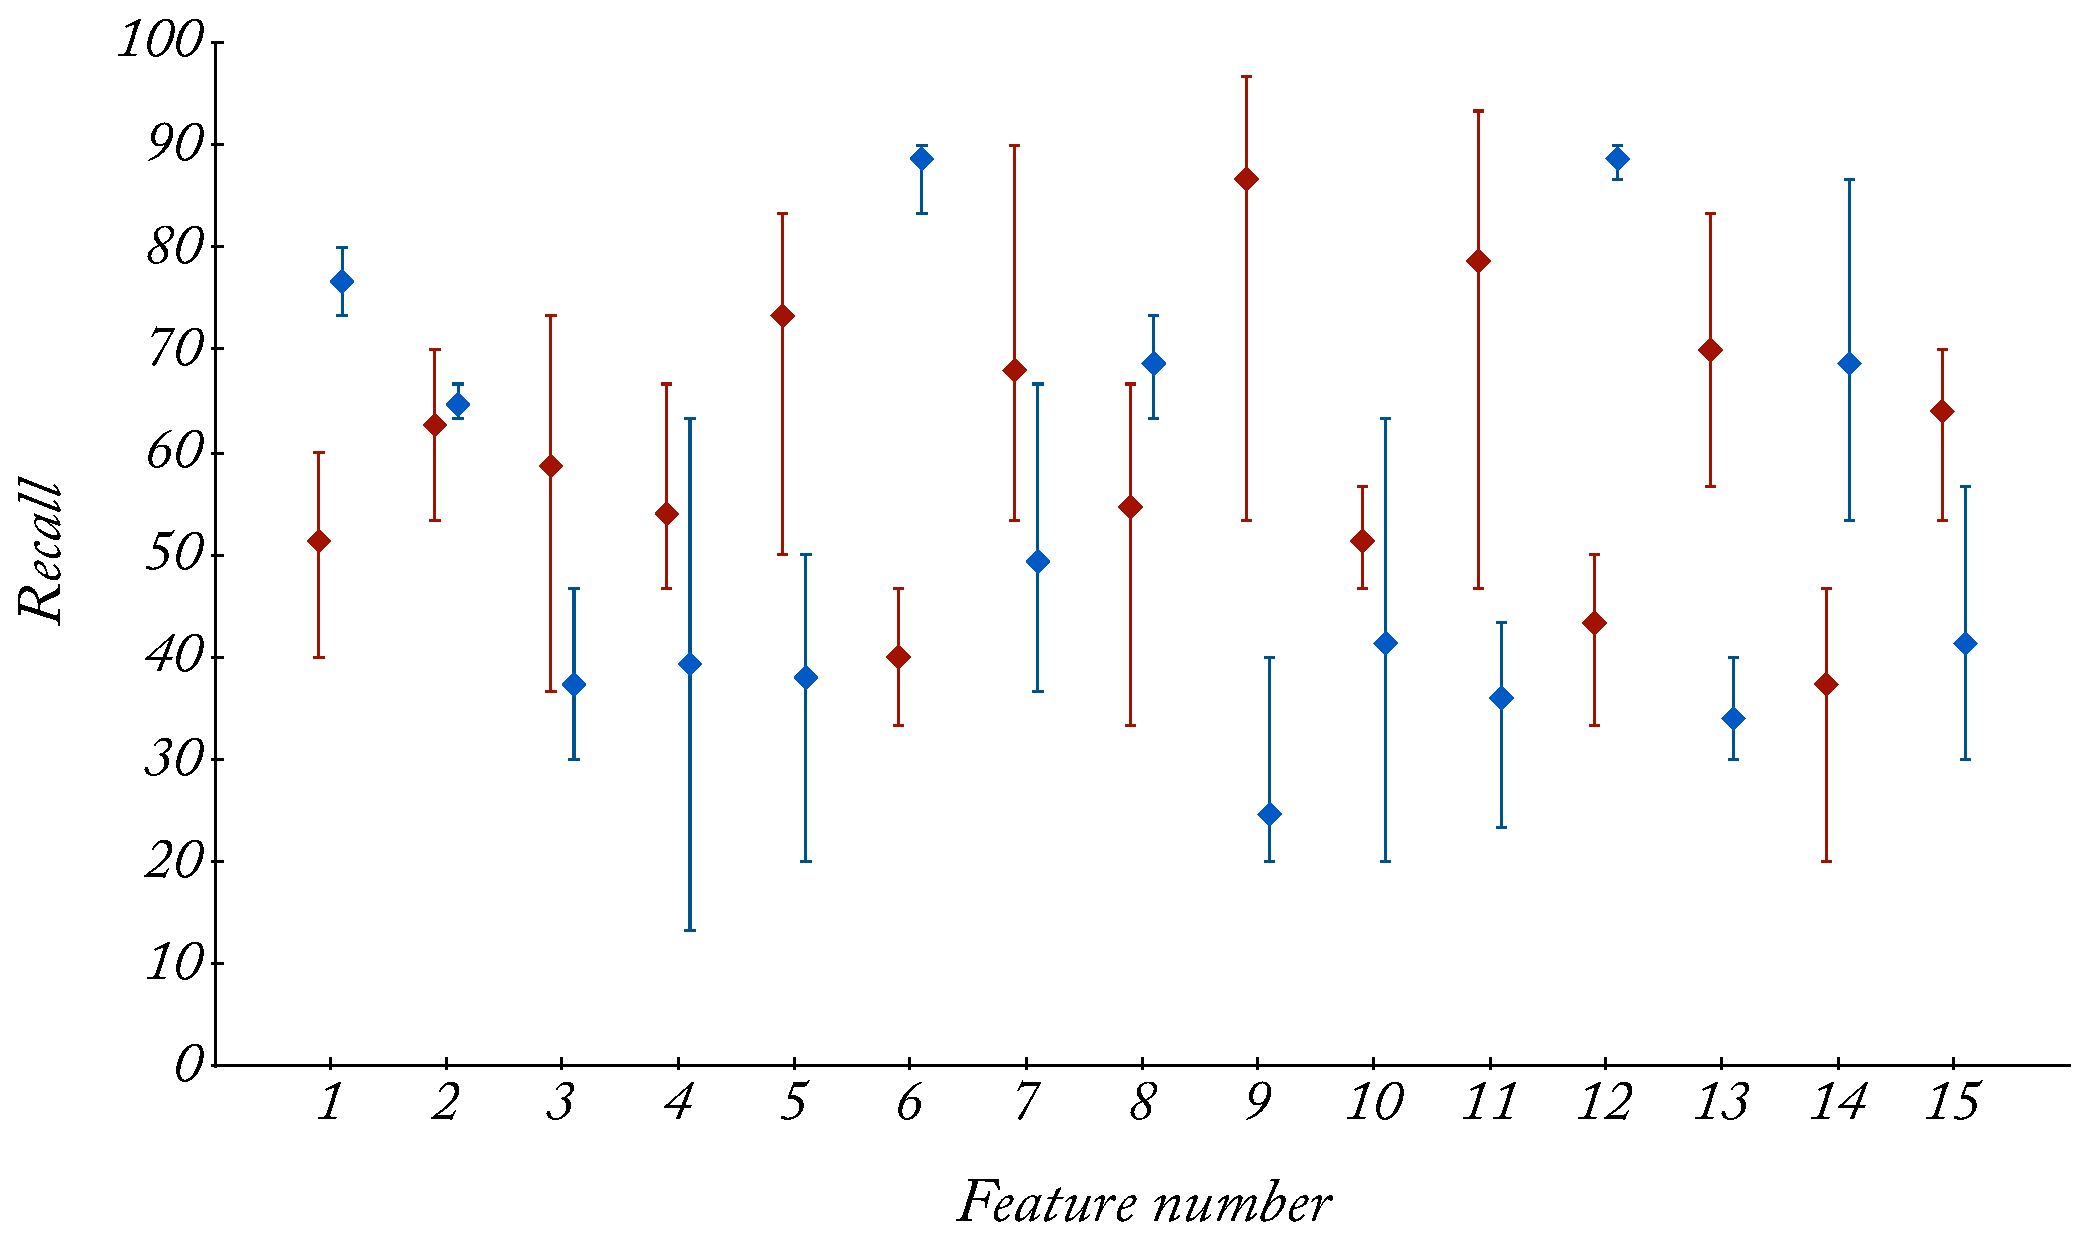
\includegraphics[width=1.0\textwidth]{graphs/polarity_r.pdf}
\end{figure}

Our recall results again highlight clue presence and strong clue-based features as particularly useful within classification. Interestingly, our pattern matched clues havea very low recall, confirming the fact that although their precision is high, their ability to classify slightly more uncertain data is low.

\subsection{Feature set performance}
\label{polarity:feature_set}

As a result of our individual feature analysis, we put forward five feature-combinations for further testing:

\begin{enumerate}
    \item has
		positive\-\_clues?, has\-\_negative\-\_clues?, has\-\_strong\-\_positive\-\_clues?, has\-\_strong\-\_negative\-\_clues?
    \item has\-\_positive\-\_clues?, has\-\_negative\-\_clues?, no\-\_strong\-\_positive\-\_clues, no\-\_strong\-\_negative\-\_clues
		\item has\-\_positive\-\_clues?, has\-\_negative\-\_clues?, has\-\_strong\-\_positive\-\_clues?, has\-\_strong\-\_negative\-\_clues?, has\-\_positive\-\_patterns?, has\-\_negative\-\_patterns?
		\item has\-\_positive\-\_clues?, has\-\_negative\-\_clues?, has\-\_strong\-\_positive\-\_clues?, has\-\_strong\-\_negative\-\_clues?, has\-\_positive\-\_patterns?, has\-\_negative\-\_patterns?, :unigrams
\end{enumerate}

The results of our tests using the five feature sets are listed in figure \ref{fig:polarity_multi}. Blue bars represent precision, red represents accuracy and green represents recall.

\begin{figure}
	\caption{Precision (square), accuracy (circle) and recall (diamond) results for our four different feature sets.}
	\label{fig:polarity_multi}
	\centering
		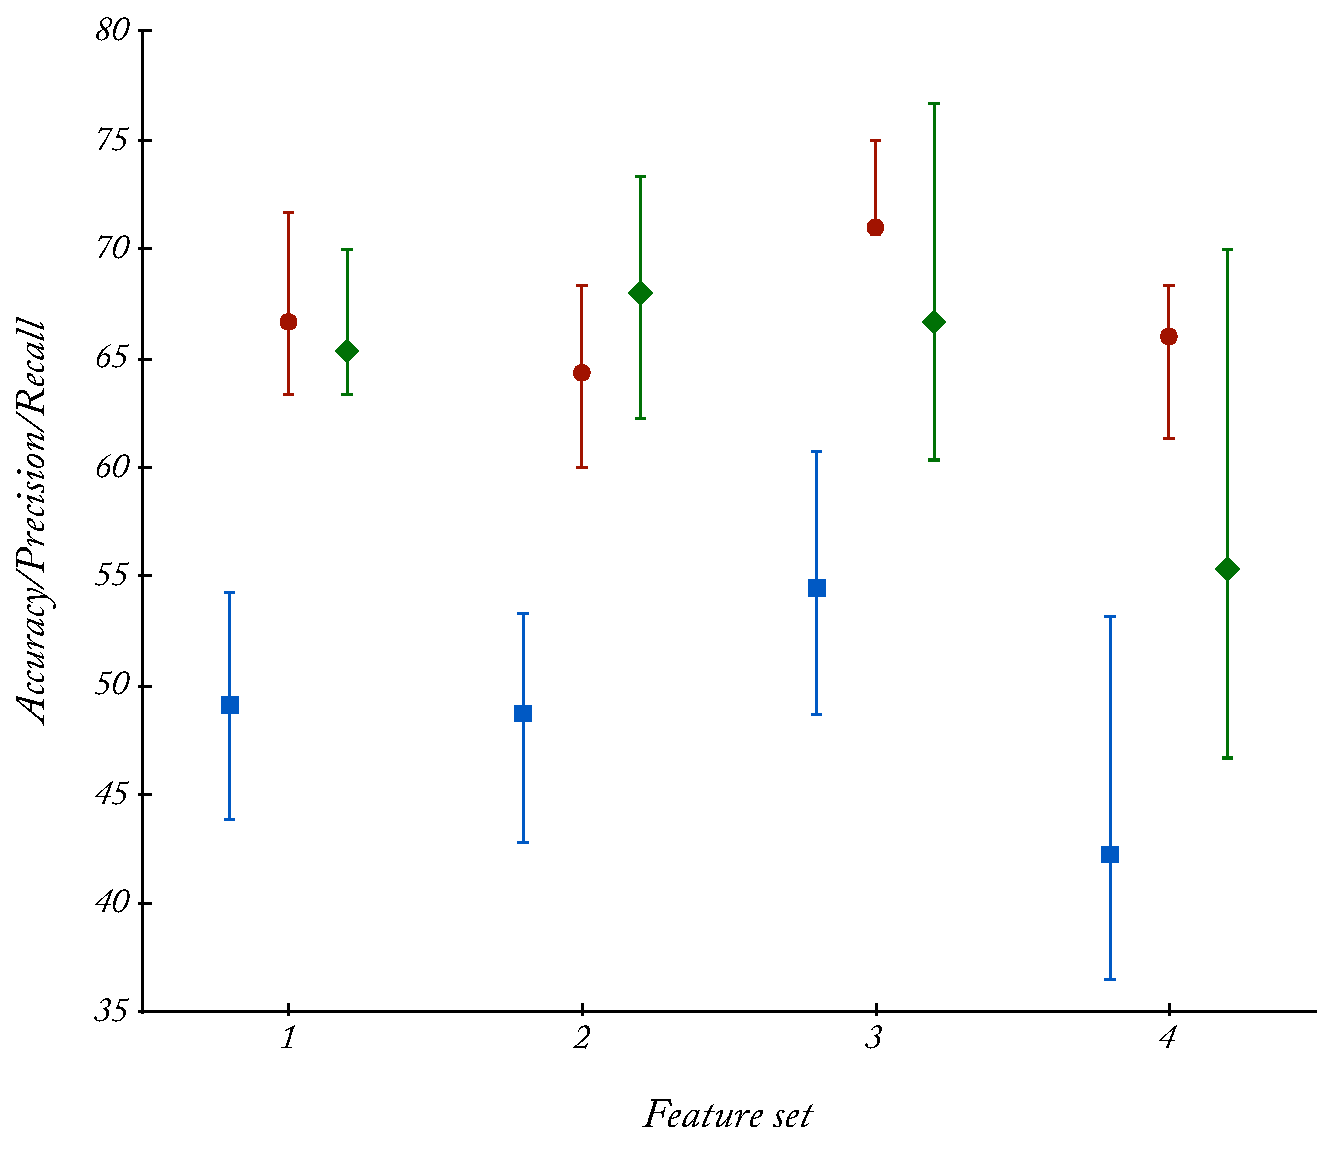
\includegraphics[width=0.9\textwidth]{graphs/polarity_multi.pdf}
\end{figure}

All classifiers perform well, however of the four, we felt that our third feature set performed the strongest. It has the highest average accuracy rate (71.0\%), along with a much stronger precision rate. Although its recall is slightly outperformed by our second feature set, overall, we still feel that it's the strongest of the feature sets. Its higher precision can probably be attributed to its use of our pattern-based features which we adapted from Turney's \cite{Turney:2002vv} original unsupervised techniques.

\subsection{Classifier type}

In order to determine the most appropriate classifier type, we ran our tests using a Support Vector Machine for one test and a Naive Bayes Classifier for the other. When building our classifiers, we used the third feature set from section \ref{polarity:feature_set}. We present our results in figure \ref{fig:polarity_class}.

\begin{figure}
	\caption{Precision (square), accuracy (circle) and recall (diamond) results for SVM and NB classifier.}
	\label{fig:polarity_class}
	\centering
		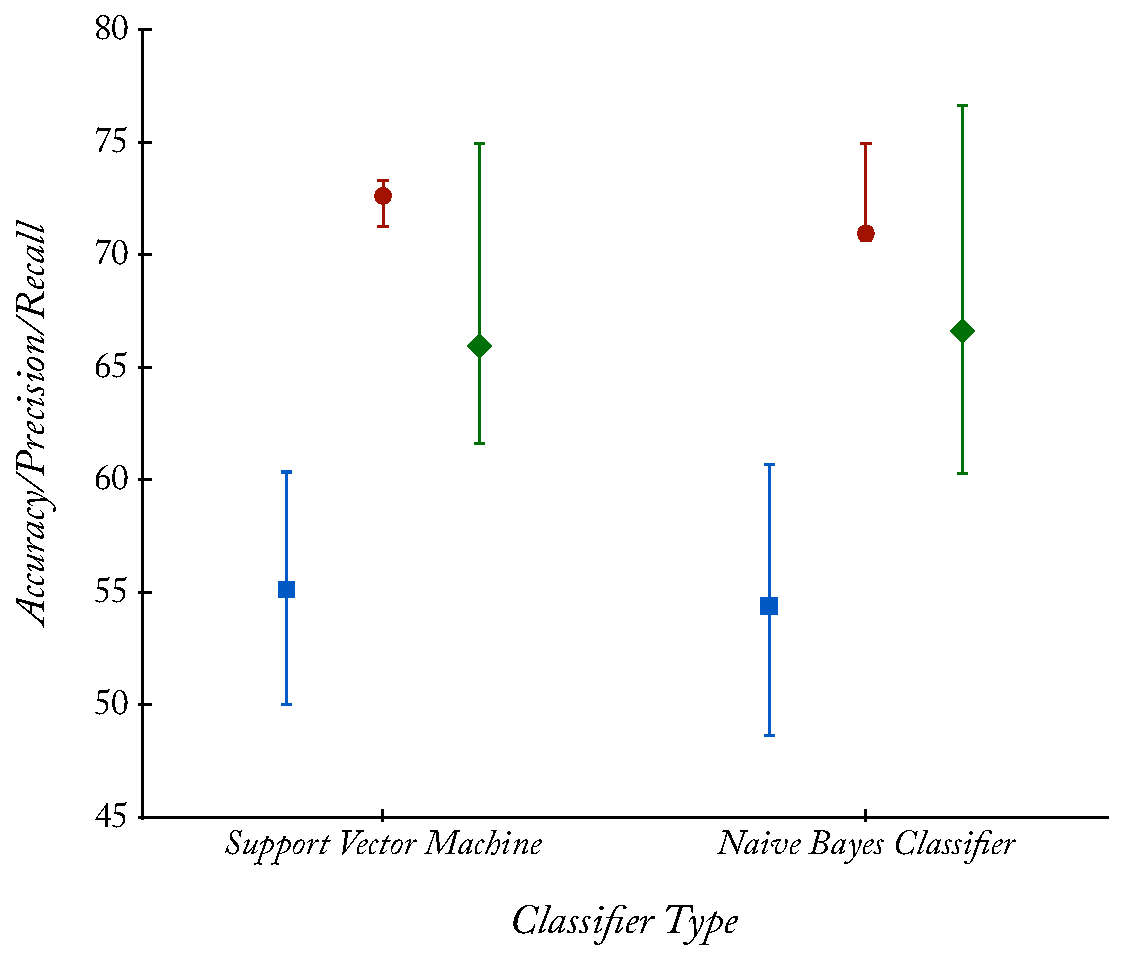
\includegraphics[width=0.8\textwidth]{graphs/polarity_class.pdf}
\end{figure}

Although both the SVM and NB classifiers perform strongly, the SVM's average accuracy of of 72.6\% against the NB classifier's 71\% make it the better classification method. Furthermore our SVM achieves a much stronger average precision that the NB classifier, and only performs marginally worse in terms of recall.

\section{Evaluation}

Overall our polarity classification performed well, achieving an avergae accuracy of 72.6\%. Our results were on par with typical research averages, only being outperformed by Barbosa et al. \cite{Barbosa:ws} who achieved rates of 74.9\%. We felt however, that this was largely due to differences in training data size. As with our subjectivity classification, we believe that with a larger training set we might have seen an improvement in overall classification rates.

In future work there are a few areas we would look to for further improvement,

\begin{description}
	\item [Training set size] - as discussed briefly above and in chapter \ref{subjectivity}, we felt that the size of our training set has a negative overall impact on classification rates, and in future would spend more time on assembling a larger set.
	\item [Word-sense disambiguation] - as discussed in chapter \ref{subjectivity}, we feel that word-sense disambiguation would in future help further improve out results.
	\item [Neutral classification] - Our approach to sentiment analysis focussed on positive and negative classification, however on occasions we felt that opinionated data presented no actual polarised opinion. Accordingly, future work might look at how we can introduce a third label for neutrality.
\end{description}

